% Shared typography for the Curious Signals topic papers.
\documentclass[journal]{IEEEtran}
\usepackage[T1]{fontenc}
\usepackage[utf8]{inputenc}
\usepackage{lmodern}
\usepackage{amsmath,amssymb,bm}
\usepackage{graphicx,booktabs,array}
\usepackage{siunitx}
\usepackage{tikz}
\usetikzlibrary{arrows.meta,positioning,calc,decorations.pathmorphing}
\usepackage{pgfplots}
\usepgfplotslibrary{groupplots}
\pgfplotsset{compat=1.18}
\usepackage{cite,microtype}
\usepackage[hidelinks]{hyperref}
\usepackage{xurl}
\definecolor{csblue}{HTML}{245B78}
\definecolor{csred}{HTML}{B65338}
\definecolor{csteal}{HTML}{278078}
\definecolor{csgold}{HTML}{967135}
\definecolor{csgray}{HTML}{62676C}
\renewcommand{\unit}[1]{\ensuremath{\,\mathrm{#1}}}
\newcommand{\code}[1]{\texttt{#1}}
\newcolumntype{P}[1]{>{\raggedright\arraybackslash}p{#1}}
\newcommand{\sourcecommit}{0a5cf6f}
\newcommand{\editiondate}{October 27, 2026}
\newcommand{\paperauthors}{Sebastian J. Spicker, Alexander K\"upper}
\pgfplotsset{every axis/.append style={
  width=0.98\columnwidth,height=4.8cm,
  label style={font=\footnotesize},tick label style={font=\scriptsize},
  legend style={font=\footnotesize,draw=none,fill=white},
  axis line style={black!65},tick style={black!65},
  grid style={black!12},major grid style={black!12},
  scaled ticks=false,
  unbounded coords=jump,
  axis on top,
  axis background/.style={fill=white}
}}
\tikzset{>=Latex,every node/.style={font=\footnotesize}}
\setlength{\emergencystretch}{1em}
\newcommand{\dataprovenance}{Data provenance: the datasets analysed in this
  paper are deterministic example data, generated for the October 2026 edition from fixed
  seeds by the scripts in \texttt{example-data/}. They are modelled on the named
  sensors' units, sampling, resolution, noise and limits; they are not
  recordings from the original work. The date above is the author's
  approximate dating of that work, not of these data.}
\newcommand{\makepapertitle}{%
  \hypersetup{pdftitle={\papertitle},pdfauthor={\paperauthors},
    pdfsubject={Measurements and laboratory models; \paperperiod; collected edition \editiondate},
    pdfkeywords={physics education, instrumentation, calibration, uncertainty, phyphox}}%
  \title{\fontsize{21}{25}\selectfont\papertitle}%
  \author{Sebastian~J.~Spicker, Alexander~K\"upper\\[0.5ex]
    {\normalsize Institute of Physics Education\\University of Cologne, Germany
      \quad\textperiodcentered\quad\paperperiod}\thanks{\dataprovenance}}%
  \markboth{Curious Signals --- Measurements and Laboratory Models}%
    {Spicker and K\"upper: \papershorttitle}%
  \maketitle
}

\usepackage{flafter}
\newcommand{\papertitle}{Laboratory Transit Photometry: Calibration, Temporal Resolution and Visible-Area Models}
\newcommand{\papershorttitle}{Laboratory Transit Photometry}
\newcommand{\paperperiod}{September 2024}
\newcommand{\experimentfile}{experiments/astronomy/transitmethode.phyphox}
\begin{document}
\makepapertitle
\begin{abstract}
A laboratory transit is an inverse problem involving visible area, surface brightness and detector response. A common measurement model connects phone, SensorTag, photocell--multimeter and Nano examples to tests of temporal resolution and to more complex occultations. Local deficits in three independent acquisition examples are 3.95, 3.99 and 4.00\%; a shallow Nano sequence gives 4.26\%, whereas a whole-record extrema estimator gives 19.30\%. A separate sampling example shows why a nominally adequate cadence can still miss a short feature: six of sixteen coarse sampling phases contain no reading in a half-second decrement. Planet--moon overlap and the occultation of a dark source patch both produce upward anomalies, but through different changes in the brightness integral. Their example contrasts are 1.48 and 2.92 percentage points, respectively. A sequence with two luminous bodies adds unequal eclipse depths of 31.05 and 10.49\% and a 29.995-s recurrence estimate. These quantities support different physical inferences; none permits a universal conversion from a light-curve minimum to an object radius.
\end{abstract}
\begin{IEEEkeywords}
Transit photometry, optical calibration, temporal resolution, correlated noise, mutual occultation, starspots, eclipsing binaries.
\end{IEEEkeywords}

\section{The inverse problem shared by the experiments}
An opaque object moving across a lamp makes the transit method accessible without astronomical distances or faint targets. The visible dip is nevertheless only the first observable. Its depth, duration and recurrence depend on different parts of the apparatus, and a change in any one of them need not imply a change in the object's radius. The useful laboratory question is therefore which properties of the optical configuration remain identifiable from the recorded signal.

Video-aided light-curve analysis\cite{transit2024} provides an independent view of the source, occulter and supports. It can establish whether the smaller silhouette is completely inside the luminous disc, whether its projected area remains approximately constant during a selected plateau, and whether a motor housing contributes to the shadow. These observations constrain an interpretation that the integrated light curve alone cannot determine. The same strategy extends to a moon carried around the model planet\cite{exomoonlesson2023}, a dark patch attached to the emitting surface, or a second luminous body.

We develop these configurations within a single brightness model. Independent detector examples first establish the distinction between a local signal deficit and a physical flux ratio. A separate optical sequence then examines the amplitude and time coverage of short features. Finally, two kinds of upward anomaly and alternating binary minima test what changes when the source is nonuniform or the companion emits light. The records have their own baselines, clocks and geometries. Similar numerical depths across them do not constitute a detector accuracy comparison, and superposing traces does not synchronize the physical events.

\begin{figure*}[t]
\centering
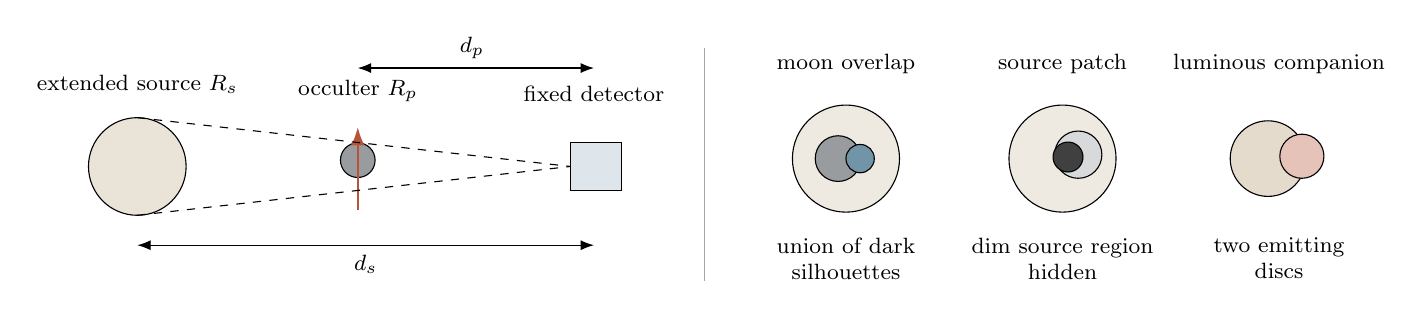
\begin{tikzpicture}[x=1cm,y=1cm]
\draw[fill=csgold!20] (1,0) circle (0.62);
\node[above] at (1,0.8) {extended source $R_s$};
\draw[fill=csgray!65] (3.8,0.08) circle (0.22);
\node[above] at (3.8,0.7) {occulter $R_p$};
\draw[->,csred,thick] (3.8,-0.55)--(3.8,0.5);
\draw[fill=csblue!15] (6.5,-0.3) rectangle (7.15,0.3);
\node[above] at (6.8,0.7) {fixed detector};
\draw[dashed] (1,0.62)--(6.5,0);
\draw[dashed] (1,-0.62)--(6.5,0);
\draw[<->] (1,-1)--(6.8,-1);
\node[below] at (3.9,-1) {$d_s$};
\draw[<->] (3.8,1.25)--(6.8,1.25);
\node[above] at (5.25,1.25) {$d_p$};
\draw[black!35] (8.2,-1.45)--(8.2,1.5);
\node[above] at (10.0,1.05) {moon overlap};
\draw[fill=csgold!15] (10,0.1) circle (0.68);
\draw[fill=csgray!65] (9.9,0.1) circle (0.29);
\draw[fill=csblue!65] (10.18,0.1) circle (0.18);
\node[below,align=center] at (10,-0.78) {union of dark\\silhouettes};
\node[above] at (12.75,1.05) {source patch};
\draw[fill=csgold!15] (12.75,0.1) circle (0.68);
\draw[fill=csgray!25] (12.95,0.15) circle (0.3);
\draw[fill=black!75] (12.82,0.12) circle (0.19);
\node[below,align=center] at (12.75,-0.78) {dim source region\\hidden};
\node[above] at (15.5,1.05) {luminous companion};
\draw[fill=csgold!25] (15.36,0.1) circle (0.48);
\draw[fill=csred!35] (15.79,0.13) circle (0.28);
\node[below,align=center] at (15.5,-0.78) {two emitting\\discs};
\end{tikzpicture}
\caption{Common apparatus and configuration insets. The detector integrates the visible, projected brightness. Distances are measured from the detector, and supports remain outside the source silhouette. Moon overlap changes the union of dark areas; a source patch changes the brightness being blocked; a luminous companion changes both the obscured contribution and the unobscured denominator.}
\label{fig:trc-apparatus}
\end{figure*}

\section{Visible brightness, projection and detector response}
\subsection{A common forward model}
Let $J_j(\lambda,\bm{x},t)$ denote the image-plane brightness of luminous body $j$, and let $\Omega_j^{\rm vis}(t)$ be its visible projected region after occultation. A detector with fixed spectral weighting $w(\lambda)$ receives a contribution proportional to
\begin{equation}
\mathcal{L}(t)=\int w(\lambda)\sum_j\int_{\Omega_j^{\rm vis}(t)}
J_j(\lambda,\bm{x},t)\,d^2x\,d\lambda.
\label{eq:trc-brightness}
\end{equation}
The projection includes the source--detector geometry. For an opaque dark planet, only the luminous source enters the sum, while its visible domain excludes the planetary silhouette. For two emitting bodies, each contributes its own brightness over whichever part remains visible. A dark surface patch modifies $J$ itself rather than adding a second foreground body.

Within a linear operating range, a useful measurement model is
\begin{equation}
X_i=D+g\int h_i(t_i-\tau)\mathcal{L}(\tau)\,d\tau+\epsilon_i,
\qquad \int h_i(u)\,du=1.
\label{eq:trc-response}
\end{equation}
Here $D$ is the additive background in signal units, $g$ is a constant response factor, $h_i$ is the temporal response kernel, and $\epsilon_i$ represents residual fluctuations. A source-blocked observation must reproduce the relevant ambient illumination and detector state if it is to estimate $D$. A covered-sensor offset and the room background are not automatically the same quantity.

The response kernel precedes notification and display. It can include optical integration and other averaging. Notification timestamps specify when readings are reported; they do not measure that kernel. Finite integration rounds a sharp ingress and can bias parameters retrieved with an instantaneous transit model\cite{kipping2010}. Subsequent averaging adds another kernel. Conversely, discarding samples changes time coverage without reproducing a slower detector's integration or filtering.

\subsection{The area-ratio special case}
For a uniform source and a smaller opaque silhouette fully inside its disc, the brightness integral reduces to an area ratio. With small angular sizes and physical radii and distances defined in Fig.~\ref{fig:trc-apparatus},
\begin{equation}
\delta=\left(\frac{R_p d_s}{R_s d_p}\right)^2,
\qquad R_p=R_s\frac{d_p}{d_s}\sqrt{\delta}.
\label{eq:trc-radius}
\end{equation}
The quantity $\sqrt{\delta}$ is directly an angular or projected radius ratio, not generally $R_p/R_s$. A physical radius requires measured $R_s$, $d_s$ and $d_p$. A grazing trajectory, transparency or a brightness gradient changes the inverse problem before any statistical uncertainty is considered.

Stellar transit models account for limb darkening\cite{mandelagol}; the same reasoning requires a laboratory source to have a measured or otherwise justified brightness distribution. The clear, red, green and blue channels of the APDS-9960 are also spectrally weighted detector outputs with programmable gain and integration\cite{apds9960}. They do not directly supply a bolometric intensity map or a resolved spectrum. A stable source spectrum and fixed detector acceptance are conditions of the simple relative-photometry model. Check for clipping and verify response proportionality over the interval spanning baseline and plateau; a nonclipped trace alone does not establish linearity.

The alternative acquisition paths impose related conditions. A phone ambient-light response depends on its sensor and processing; the SensorTag supplies another ambient-light observable. A photocell attached to a multimeter supplies voltage. Before a normalized voltage is treated as a flux ratio, its transfer must be established at the actual load, temperature and light level. Reference-cell work at low irradiance\cite{hamadani2020} illustrates why electrical operating conditions belong in an optical calibration rather than being absorbed into a dimensionless ratio.

\section{Local baselines across four acquisition examples}
\subsection{One estimator, explicit background conventions}
Let $B$ be an unobscured local mean and $P$ the corresponding plateau mean. Under the conditions of Eq.~\ref{eq:trc-response}, the background-subtracted deficit is
\begin{equation}
\widehat\delta=\frac{B-P}{B-D},\qquad B>D.
\label{eq:trc-depth}
\end{equation}
A normalization is useful only insofar as its reference represents the intended physical state. Ignoring a positive background dilutes the inferred source deficit: if $D$ is the true additive contribution, then $(B-P)/B=\delta(B-D)/B$. An incorrect baseline can instead move the entire normalized unobscured trace away from unity. Neither effect is repaired by collecting more samples of the same biased reference.

Three acquisition examples contain events near their own record times $c=22$, 52 and $82\unit{s}$. For each event, $B$ is the mean over samples satisfying $3\leq|t-c|<6\unit{s}$ and $P$ is the mean over samples with $|t-c|\leq1\unit{s}$. The reported observable for this reduction is the unsubtracted signal deficit $1-P/B$. The arithmetic mean of the three event deficits is 3.948\% for the SensorTag, 3.993\% for the phone and 3.997\% for the photocell--multimeter. For the photocell--multimeter, conversion of the voltage deficit to an optical flux deficit depends on the load-specific transfer.

\begin{figure}[t]
\centering% Canonical photometry comparison; existing prepared tables are unchanged.
\begin{tikzpicture}
\begin{groupplot}[group style={group size=1 by 2,vertical sep=1.0cm},
width=0.96\columnwidth,height=3.8cm,grid=major,enlarge x limits=false,
legend style={font=\scriptsize,at={(0.5,1.03)},anchor=south,legend columns=3,draw=none,fill=none},
title style={font=\scriptsize,at={(0.02,0.98)},anchor=north west,fill=white},
label style={font=\footnotesize},tick label style={font=\scriptsize}]
\nextgroupplot[ylabel={Signal / baseline},xmin=18,xmax=26,ymin=0.95,ymax=1.015,title={(a) Independent record times (s)}]
\addplot[csblue,solid,line width=0.8pt,mark=*,mark size=0.7pt] table[col sep=comma,x=c0,y expr={\thisrow{c1}*0.00117392937641}] {data/transitmethode_sensortag.csv};
\addlegendentry{Tag}
\addplot[csred,dashed,line width=0.8pt] table[col sep=comma,x=c0,y expr={\thisrow{c1}*0.00191565514951}] {data/transitmethode_phone.csv};
\addlegendentry{Phone}
\addplot[csteal,dashdotted,line width=0.8pt,mark=*,mark size=0.6pt] table[col sep=comma,x=c0,y expr={\thisrow{c1}*0.53828556049}] {data/transitmethode_owon.csv};
\addlegendentry{Cell voltage}
\nextgroupplot[ylabel={Nano clear (count)},xmin=10,xmax=90,xlabel={Nano receive time (s)},title={(b) Three shallow transits}]
\addplot[csblue,solid,opacity=0.25,line width=0.5pt] table[col sep=comma,x=c0,y expr={\thisrow{c2}}] {data/drafts/nano-transit.csv};
\addlegendentry{Raw}
\addplot[csred,dashed,line width=0.9pt] table[col sep=comma,x=c0,y expr={\thisrow{c1}}] {data/drafts/nano-transit-blocks.csv};
\addlegendentry{1 s means}
\end{groupplot}
\end{tikzpicture}

\caption{Upper: first events from the independent SensorTag, phone and photocell--multimeter records, each normalized by its local baseline. The photocell trace is a voltage ratio. Lower: raw clear counts and one-second means for the separate shallow Nano sequence.}
\label{fig:trc-paths}
\end{figure}

\begin{table}[t]
\caption{Transit signal deficits, cadence, threshold spans and recurrence from four independent acquisition paths. Tag, phone and cell use unsubtracted signal ratios; Nano uses a 10-count background and receive-clock spacing. Dashes identify unassigned timing.}
\label{tab:trc-paths}
\centering\footnotesize\setlength{\tabcolsep}{3pt}
\begin{tabular}{@{}lrrrr@{}}\toprule
Quantity & Tag & Phone & Cell & Nano\\\midrule
Median spacing (s)&0.800&0.09985&0.500&0.05043\\
Local deficit (\%)&3.948&3.993&3.997&4.260\\
Extrema deficit (\%)&5.267&5.223&4.357&19.298\\
Mean interval (s)&30.000&30.009&30.000&---\\
Mean span (s)&2.933&3.198&3.500&---\\\bottomrule
\end{tabular}
\end{table}

\subsection{A shallow Nano sequence tests reference choice}
The Nano events occur around device times $c=20$, 50 and $80\unit{s}$. Their primary reduction uses baseline windows $[c-6,c-3)$ and $[c+3,c+6)$, with plateau windows $[c-1,c+1)\unit{s}$. Device time selects samples associated with the signal; the separate receive time is retained for plotting. The adopted background is 10 counts. This reduction treats the dark offset as an adopted parameter.

The three local baseline means are 115.14, 115.28 and 115.25 counts, whereas the plateau means are 111.33, 110.23 and 110.68 counts. Their deficits are 3.63, 4.80 and 4.35\%, giving a mean of 4.26\% and an event-to-event standard deviation of 0.59 percentage points. That standard deviation describes the repeatability of three window reductions. It is not a confidence interval obtained from the total number of recorded readings.

The mean local baseline, 115.22 counts, also exposes the difference between a measured state and an entered normalization. The adopted reference of 110 counts gives an unobscured normalized level of 1.0522 under the same 10-count subtraction. This normalization places the measured unobscured level above unity. Re-estimating the local baseline addresses that particular discrepancy while leaving the adopted background and detector linearity as separate assumptions.

A whole-record extrema estimator, $(X_{\max}-X_{\min})/(X_{\max}-D)$, gives 19.30\% for the Nano sequence. Its baseline sample scatter is 2.72--2.81 counts, compared with local mean deficits of only 3.82--5.05 counts. Selecting the highest and lowest samples from a long record accentuates those fluctuations and does not compare equivalent optical states. The smaller extrema excesses in the three other examples have the same statistical vulnerability. Their different magnitudes cannot be used to rank detector accuracy because the examples have independent signal levels, noise and timing.

Within the uniform-source model, the Nano mean deficit corresponds to $\sqrt{\delta}=0.2064$. Conversion to a physical planet radius additionally depends on the geometry in Eq.~\ref{eq:trc-radius}. Even the projected ratio inherits the uncertainty and model dependence of the adopted background. The estimator, adopted background and physical geometry jointly determine the radius interpretation.

\subsection{Uncertainty belongs to the shared reference}
For Eq.~\ref{eq:trc-depth}, the sensitivity vector with respect to $(B,P,D)$ is
\begin{equation}
\begin{aligned}
\bm{a}&=\left(\frac{P-D}{(B-D)^2},\ -\frac{1}{B-D},
\frac{B-P}{(B-D)^2}\right),
\\
 u^2(\delta)&=\bm{a}\,\bm{\Sigma}\,\bm{a}^{\mathsf T},
\end{aligned}
\label{eq:trc-uncertainty}
\end{equation}
where $\bm{\Sigma}$ contains their variances and covariances. A common baseline or background couples all normalized points. Photometric covariance can therefore dominate an apparent improvement obtained by increasing the point count\cite{pont2006}. The relevant averaging behaviour must be examined over the duration of the event or anomaly, not inferred solely from adjacent-sample scatter.

If a physical radius is justified, the logarithmic sensitivity is $d\ln R_p=d\ln R_s+d\ln(d_p/d_s)+\tfrac12d\ln\delta$. Independent contributions can be combined in quadrature only when their independence is defensible; otherwise the geometry and depth covariances remain. A changing source brightness map is a model error, not an additional independent count fluctuation. A known second silhouette, a separately measured background and a load-specific optical transfer each constrain a different part of this inference.

\section{Temporal resolution: cadence, integration and noise}
\subsection{A delivered sequence has two clocks}
The shallow Nano sequence has median device and receive intervals of 0.05000 and $0.05043\unit{s}$. Those numbers describe that sequence, not an optical bandwidth. A separate detector-characterization example makes the clock distinction more visible. Adjacent differences of its device timestamps have mean $50.340\unit{ms}$ and sample standard deviation $0.474\unit{ms}$. Receive intervals have a similar mean, $50.344\unit{ms}$, but a $4.245\unit{ms}$ standard deviation. The receive-interval scatter is about nine times larger even though the mean rates agree closely.

The reciprocal mean device interval is $19.8649\unit{Hz}$. Association of each device reading with its notification permits the two spacing series to be compared against the device time of the later sample, as in Fig.~\ref{fig:trc-sampling}. It does not synchronize the clocks or establish an absolute latency. A missed notification should remain a gap in elapsed receive time. Replacing measured times with sample number times a nominal period would obscure that distinction.

\begin{figure}[t]
\centering% Canonical photometry comparison; existing prepared tables are unchanged.
\begin{tikzpicture}
\begin{groupplot}[group style={group size=1 by 2,vertical sep=1.0cm},
width=0.96\columnwidth,height=3.8cm,grid=major,enlarge x limits=false,
legend style={font=\scriptsize,at={(0.5,1.03)},anchor=south,legend columns=3,draw=none,fill=none},
title style={font=\scriptsize,at={(0.02,0.98)},anchor=north west,fill=white},
label style={font=\footnotesize},tick label style={font=\scriptsize}]
\nextgroupplot[ylabel={Clear (count)},xmin=29,xmax=49,ymin=920,ymax=1060,title={(a) Feature windows; device time (s)}]
\addplot[csblue,solid,line width=0.6pt] table[col sep=comma,x=c0,y expr={\thisrow{c2}}] {data/drafts/detector-characterization.csv};
\nextgroupplot[ylabel={Interval (ms)},xmin=0,xmax=60,xlabel={Device time of later sample (s)},title={(b) Adjacent notification intervals}]
\addplot[csblue,solid,line width=0.6pt] table[col sep=comma,x=c0,y expr={\thisrow{c1}}] {data/drafts/optics-detector-intervals.csv};
\addlegendentry{Device}
\addplot[csred,dashed,line width=0.6pt] table[col sep=comma,x=c0,y expr={\thisrow{c2}}] {data/drafts/optics-detector-intervals.csv};
\addlegendentry{Receive}
\end{groupplot}
\end{tikzpicture}

\caption{Upper: short decrements on device time. Lower: device and receive intervals plotted at the later device timestamp. Receive-interval scatter is about nine times larger, while mean intervals agree closely.}
\label{fig:trc-sampling}
\end{figure}

An integration kernel changes the continuous shape before these spacings are considered. Ingress and egress become rounded; the apparent interval between crossings depends on the kernel as well as the chosen threshold. The finite-exposure analysis of Kipping\cite{kipping2010} supplies the astronomical counterpart. In the laboratory, reducing the model's speed while holding detector settings fixed tests whether the recovered shape or depth is limited by temporal response. A high notification rate alone cannot establish that test's outcome.

\subsection{The amplitude budget is not a detection probability}
In the characterization example, the illuminated device-time interval $12\leq t\leq28\unit{s}$ contains 318 readings with mean $\mu=1022.736$ counts and sample standard deviation $s=10.636$ counts. The dark interval $0\leq t<9\unit{s}$ has mean 11.156 counts. The accompanying numerical summary reproduces the directly calculated interval and baseline quantities to its rounding precision, including the baseline count.

For a proposed fractional decrement $\delta$, a planning amplitude ratio is
\begin{equation}
\rho_1=\frac{\delta(\mu-D)}{s}.
\label{eq:trc-snr}
\end{equation}
The summary's 2\% proposal uses an entered dark value of 8 counts, giving a 20.295-count decrement and $\rho_1=1.908$. That entered value is distinct from the observed dark mean. The event reductions below instead use the latter in the denominator. The planning and event reductions therefore use different stated background conventions.

The baseline's lag-one correlation is 0.055, and the standard deviation of sixteen one-second block means is 2.64 counts. These are diagnostics over one finite interval. They do not establish stationarity at longer times or a universal square-root law for uncertainty. In particular, $\rho_1$ is not a false-alarm probability, a fitted event significance or an uncertainty of a mean. Lamp flicker and mechanical repetition can create covariance on timescales quite different from one sample\cite{pont2006}.

\begin{table}[t]
\caption{Feature depths and single-reading amplitude ratios in half-open device-time windows. Coarse $N$ gives the sample-count range across all sixteen phases of retaining every sixteenth reading.}
\label{tab:trc-sampling}
\centering\footnotesize\setlength{\tabcolsep}{3.5pt}
\begin{tabular}{@{}lrrrr@{}}\toprule
Window (s)&$N$&Depth (\%)&$\rho_1$&Coarse $N$\\\midrule
$[30,30.5)$&10&0.61&0.58&0--1\\
$[34,35)$&20&2.29&2.18&1--2\\
$[38,40)$&40&3.98&3.78&2--3\\
$[44,48)$&79&7.86&7.47&4--5\\\bottomrule
\end{tabular}
\end{table}

\subsection{Sampling phase can remove a feature entirely}
The first feature contains ten readings in its half-second window, yet its mean deficit is only 0.61\% of the background-subtracted illuminated level. The progressively longer features have mean deficits of 2.29, 3.98 and 7.86\% (Table~\ref{tab:trc-sampling}). These are measured means over the stated feature windows. The shallow first feature is difficult to distinguish from the baseline scatter even before time coverage is reduced.

Retaining every sixteenth sample gives a spacing near $0.805\unit{s}$. Counting retained readings in each unchanged feature window for all sixteen possible starting phases shows that six phases miss the half-second feature completely; the remaining ten contain one reading each. The one-second feature retains one or two readings, while the four-second feature retains four or five. These counts use the actual time boundaries, not a duration divided by a rounded mean rate.

Decimation does not reproduce a slower instrument. Its integration, anti-alias filtering, sensitivity and noise may all differ. The calculation isolates temporal coverage: a large decrement would still be absent from a phase that contains no sample. Averaging groups would ask a different question by spreading a short decrement across a longer response window. Thus amplitude, time coverage and integration need separate checks. A nominal rate chosen relative to the planet's slow orbital repetition can be adequate for recurrence while failing to resolve a much shorter moon or spot feature.

\section{Threshold spans and recurrence are different observables}
The original three-path examples illustrate this distinction without fitting an orbital model. For each event, consider readings with $|t-c|<3\unit{s}$ and a threshold of $0.98B_k$, using that event's local baseline. The onset is the first below-threshold sample in this window. The end is the first recovered sample after the last below-threshold sample in the window. This windowed span includes any intervening recrossings and uses no interpolation. It should not be identified with geometric first-to-fourth contact or with a differently configured live hysteresis rule.

The resulting mean spans are 2.933, 3.198 and $3.500\unit{s}$ for SensorTag, phone and photocell--multimeter, respectively. Their mean onset intervals are nevertheless 30.000, 30.009 and $30.000\unit{s}$. The SensorTag's individual intervals are 30.4 and $29.6\unit{s}$ on its 0.8-s example grid, while the phone gives 30.073 and $29.945\unit{s}$. Similar mean recurrence therefore coexists with visibly different threshold spans and interval quantization. These differences do not establish which detector is more accurate in a common experiment.

Three events give two adjacent intervals, whose mean is
\begin{equation}
\overline T=\frac{(t_1-t_0)+(t_2-t_1)}{2}
=\frac{t_2-t_0}{2}.
\label{eq:trc-period}
\end{equation}
The middle onset cancels. Shared endpoints correlate the adjacent intervals, so their apparent scatter cannot be treated as independent replicated timing errors. Delivery latency, finite integration and threshold choice can shift onsets relative to the physical event even when the recorded timestamps are retained correctly. Conversely, a fitted transit centre and a threshold onset need not have the same uncertainty or physical interpretation.

The shallow Nano deficit is only modestly larger than its per-sample scatter, so a first isolated threshold crossing there can be a fluctuation. We therefore retain its primary window-mean depth and do not assign a new threshold period from the densely sampled sequence. The stronger binary minima below permit a separate localized onset estimate. This choice reflects the observable supported by each example, rather than applying one event detector indiscriminately.

\section{Two upward anomalies, two physical mechanisms}
\subsection{Mutual overlap recovers duplicated blocked area}
For a planet and moon fully projected onto a uniform source, let $A_p$, $A_m$ and $A_{pm}$ denote planet, moon and mutual-overlap areas in the same projection. Equation~\ref{eq:trc-brightness} becomes
\begin{equation}
F=1-\frac{A_p+A_m-A_{pm}}{A_s}.
\label{eq:trc-moon}
\end{equation}
Increasing $A_{pm}$ removes duplicated blocking from the sum and therefore increases the received light. Mutual-transit models\cite{sato2009} show this geometrical brightening; the classroom moon experiment\cite{exomoonlesson2023} makes the projected configurations visible. It is not emission by the dark companions.

Use four characteristic means: baseline $B$, planet-only $P_0$, separated silhouettes $S$ and overlap $O$. With a common background $D$, define
\begin{equation}
E=\frac{P_0-S}{B-D},\qquad
C_m=\frac{O-S}{B-D},\qquad
q=\frac{O-S}{P_0-S}.
\label{eq:trc-moon-contrast}
\end{equation}
$E$ is the resolved extra deficit and $C_m$ the overlap brightening. Under matched geometry and brightness, $q$ is the recovered fraction of the extra blocked area. Its cancellation of the common denominator removes that particular normalization sensitivity, not the need for matching silhouettes.

The primary moon reduction uses device-time windows $[3,17)$ and $[93,107)\unit{s}$ for baseline; $[22,33)$ and $[77,88)$ for planet only; $[37,48)$ and $[62,73)$ for separated silhouettes; and $[52,58)$ for overlap. Their mean clear counts are 115.33, 104.99, 102.02 and 103.58, respectively. With the adopted $D=10$ counts, the extra deficit is 2.82 percentage points and the overlap brightening is 1.48 points. The recovered fraction is $q=0.525$: only about half of the extra deficit is reversed, and the overlap level remains below the planet-only level.

\begin{figure}[t]
\centering% Canonical photometry comparison; existing prepared tables are unchanged.
\begin{tikzpicture}
\begin{groupplot}[group style={group size=1 by 2,vertical sep=1.0cm},
width=0.96\columnwidth,height=3.8cm,grid=major,enlarge x limits=false,
legend style={font=\scriptsize,at={(0.5,1.03)},anchor=south,legend columns=3,draw=none,fill=none},
title style={font=\scriptsize,at={(0.02,0.98)},anchor=north west,fill=white},
label style={font=\footnotesize},tick label style={font=\scriptsize}]
\nextgroupplot[ylabel={Moon clear (count)},xmin=32,xmax=78,ymin=90,ymax=115,title={(a) Moon: own receive time (s)}]
\addplot[csblue,solid,opacity=0.25,line width=0.5pt] table[col sep=comma,x=c0,y expr={\thisrow{c2}}] {data/drafts/exomoon-photometry.csv};
\addlegendentry{Raw}
\addplot[csred,dashed,line width=0.9pt] table[col sep=comma,x=c0,y expr={\thisrow{c1}}] {data/drafts/exomoon-photometry-blocks.csv};
\addlegendentry{1 s means}
\nextgroupplot[ylabel={Spot clear (count)},xmin=43,xmax=61,xlabel={Spot record receive time (s)},title={(b) Dark source patch}]
\addplot[csblue,solid,opacity=0.25,line width=0.5pt] table[col sep=comma,x=c0,y expr={\thisrow{c2}}] {data/drafts/starspot-crossing.csv};
\addplot[csred,dashed,line width=0.9pt] table[col sep=comma,x=c0,y expr={\thisrow{c1}}] {data/drafts/starspot-crossing-blocks.csv};
\end{groupplot}
\end{tikzpicture}

\caption{Two independent sequences produce local upward features. Moon overlap reduces the union of dark silhouettes in the upper panel; a planet hiding a dim source patch removes less brightness in the lower panel. Each panel uses its own receive clock. One-second means display the characteristic-state contrasts.}
\label{fig:trc-brightenings}
\end{figure}

\subsection{A source patch reduces the brightness being hidden}
A patch on the emitting surface changes the integrand of Eq.~\ref{eq:trc-brightness}. If the same planet area $A$ covers brightness $J_b$ outside the patch and $J_s<J_b$ over it, the recovered contribution is proportional to $A(J_b-J_s)$. The anomaly consequently constrains a covered-area--brightness-contrast product. A small dark patch and a larger weakly dim patch can produce the same integrated change. This is distinct from the union-area mechanism in Eq.~\ref{eq:trc-moon} even though both can make a positive excursion during a deficit.

The spotted-source comparison uses baseline windows $[5,15)$, $[65,75)$ and $[95,105)\unit{s}$. Adjacent plateaus use $[45.5,48.5)$ and $[55.5,58.5)$; the crossing uses $[50.5,53.5)$. Their baseline, adjacent and crossing means are 115.11, 100.05 and 103.12 counts. The local contrast,
\begin{equation}
C_s=\frac{X_{\rm cross}-X_{\rm adjacent}}{B-D},
\label{eq:trc-spot}
\end{equation}
is 2.92 percentage points with $D=10$ counts, recovering 20.4\% of the adjacent deficit. The adjacent and crossing depths remain 14.33 and 11.41\%, so the upward anomaly does not restore the unobscured level.

These windows compare settled characteristic states. The intervening returns to higher light are excluded; the entire central sequence is not fitted as a single uninterrupted geometrical crossing. Separate deeper control windows, $[20.5,23.5)$ and $[80.5,83.5)\unit{s}$, give 19.16\% deficit. They establish another observed level. Interpreting its difference from the adjacent plateau as a spot covering fraction depends on matching the two projected silhouettes.

If the adjacent and crossing depths were nevertheless inserted into the uniform-source square-root relation, their inferred projected radii would differ by a factor 0.892. This apparent 10.8\% reduction illustrates a model mismatch, not a physical radius change. Stellar calculations show how unmodelled spot anomalies can bias fitted radius, duration and timing\cite{oshagh2013}. Their quantitative corrections depend on spot location and brightness; they cannot be transferred as a universal adjustment to a lamp model.

\begin{table}[t]
\caption{Moon and source-patch contrasts from characteristic-state means, each using its local baseline and a 10-count background. Scale is the quadrature combination of one-second block SDs divided by the net baseline.}
\label{tab:trc-brightenings}
\centering\footnotesize\setlength{\tabcolsep}{3pt}
\begin{tabular}{@{}lrrr@{}}\toprule
Comparison & Change (count)&Contrast (pp)&Scale (pp)\\\midrule
Moon extra deficit&2.97&2.82&0.81\\
Moon overlap recovery&1.56&1.48&0.96\\
Spot crossing recovery&3.07&2.92&0.63\\\bottomrule
\end{tabular}
\end{table}

\subsection{What distinguishes the two explanations}
The one-second block dispersions are 0.54, 0.66 and 0.76 counts for the moon's planet-only, separated and overlapping states. Combining the relevant dispersions in quadrature and dividing by the local net baseline gives the descriptive scales in Table~\ref{tab:trc-brightenings}. The spot comparison has adjacent and crossing block dispersions of 0.50 and 0.43 counts. There are only six complete overlap blocks and three crossing blocks. Those counts are not independent physical repetitions, and the scales do not establish a detection probability.

The discrimination instead comes from controlled geometry. A moon interpretation requires separated and overlapping silhouettes, with both bodies inside the source in the compared windows. A source-patch interpretation requires the dim region to be attached to the emitting surface and a comparable planetary silhouette on either side of the anomaly. A motor-only control, a no-patch control and a detector-view image test different alternatives. A rod leaving the beam can brighten either configuration without realizing the intended astronomical mechanism.

Moon mass and spot temperature depend on dynamical and brightness information, respectively. A moon radius additionally needs a resolved fully superimposed silhouette, source scale and projection distances. Dynamical transit-timing or transit-duration variations depend on recurring orbital information in addition to the characteristic brightness means. For an identical moon phase every planetary orbit, the phase advance is $2\pi T_p/T_m$, so $T_p/T_m$ must be an integer; a rational noninteger ratio repeats only after several planetary orbits. The state sequence itself does not establish either period. Spot amplitude likewise leaves its area, brightness and track position degenerate.

\section{Two luminous bodies change the denominator}
The binary configuration makes a further alteration to the same brightness integral. For two uniform projected discs, let $J_1,J_2$ be detector-weighted surface brightnesses and $A_1,A_2$ their unobscured areas. The baseline source contribution is $L=J_1A_1+J_2A_2$. If the same overlap area $A_o$ is hidden at the two conjunctions,
\begin{equation}
\delta_1=\frac{J_1A_o}{L},\qquad
\delta_2=\frac{J_2A_o}{L}.
\label{eq:trc-binary}
\end{equation}
Only under those equal-overlap conditions would the depth ratio give $J_1/J_2$. It would still not give the total luminosity ratio without the two areas. Partial eclipses, unequal projected overlaps and source brightness structure change the relation. Modern binary calculations integrate local passband intensities over the two visible surfaces\cite{prsa2016}; the dark-planet square-root rule discards the companion's contribution to $L$.

Primary denotes the deeper observed minimum, not necessarily the eclipse of the larger object. The example primary centres are near device times 20, 50, 80 and $110\unit{s}$, and secondary centres are near 35, 65 and $95\unit{s}$. For every centre $c$, the local baseline uses $[c-6,c-3)$ and $[c+3,c+6)$, and the minimum uses $[c-0.75,c+0.75)\unit{s}$. This common central window lies inside both types of minimum. The background is the adopted 10 counts, while the local baseline replaces an entered 210-count normalization reference.

\begin{figure}[t]
\centering% Canonical photometry comparison; existing prepared tables are unchanged.
\begin{tikzpicture}
\begin{groupplot}[group style={group size=1 by 1,vertical sep=1.0cm},
width=0.96\columnwidth,height=4.5cm,grid=major,enlarge x limits=false,
legend style={font=\scriptsize,at={(0.5,1.03)},anchor=south,legend columns=3,draw=none,fill=none},
title style={font=\scriptsize,at={(0.02,0.98)},anchor=north west,fill=white},
label style={font=\footnotesize},tick label style={font=\scriptsize}]
\nextgroupplot[ylabel={Clear (count)},xmin=10,xmax=118,xlabel={Receive time (s)},title={Alternating primary and secondary minima}]
\addplot[csblue,solid,opacity=0.30,line width=0.5pt] table[col sep=comma,x=c0,y expr={\thisrow{c2}}] {data/drafts/eclipsing-binary.csv};
\addlegendentry{Raw}
\addplot[csred,dashed,line width=0.9pt] table[col sep=comma,x=c0,y expr={\thisrow{c1}}] {data/drafts/eclipsing-binary-blocks.csv};
\addlegendentry{1 s means}
\end{groupplot}
\end{tikzpicture}

\caption{Unequal alternating minima distinguish successive eclipse events from a full primary-to-primary cycle. Raw clear counts and one-second means retain the contrast between primary and secondary states; the two types also have different apparent durations.}
\label{fig:trc-binary}
\end{figure}

The four primary reductions have mean depth 31.05\% and event standard deviation 0.20 percentage points; the three secondary reductions give 10.49\% and 0.12 points. Their mean depth difference is 20.56 points and their ratio is 2.96. These are unequal removed contributions. Interpretation of the depth ratio as a brightness ratio depends on matched projected overlap areas, with the differing apparent durations providing a geometrical constraint. Component temperatures, radii and masses additionally depend on surface-brightness, geometrical and dynamical constraints.

\begin{table}[t]
\caption{Binary eclipse depths and primary-onset intervals. SD summarizes event-to-event depth variation or interval variation; adjacent intervals share endpoints.}
\label{tab:trc-binary}
\centering\footnotesize
\begin{tabular}{@{}lrr@{}}\toprule
Depth statistic & Primary & Secondary\\\midrule
Number of events&4&3\\
Mean depth (\%)&31.05&10.49\\
Event SD (percentage points)&0.20&0.12\\\midrule
\multicolumn{3}{@{}l}{Primary onset intervals (s): 29.989, 29.991, 30.005}\\
\multicolumn{3}{@{}l}{Mean interval: 29.995 s; descriptive SD: 0.008 s}\\\bottomrule
\end{tabular}
\end{table}

A separate timing reduction locates each primary onset as the first sample below the midpoint between its local baseline and minimum mean, searching only within $[c-3,c)$ on the device clock. The associated receive time supplies the onset coordinate. Its intervals are 29.989, 29.991 and $30.005\unit{s}$, with mean $29.995\unit{s}$ and sample standard deviation $0.008\unit{s}$. The strong primary deficit makes the localized crossing unambiguous in this example. Decimal resolution does not establish equivalent physical timing accuracy, and the shared endpoints again prevent treating the intervals as independent period repetitions.

The entered phase definition is $\phi=\operatorname{frac}[(t_{\rm rec}-20\unit{s})/(30\unit{s})]$. The reported phase follows this stated phase convention to numerical rounding. Folding at the separation between adjacent unequal minima would mix primary and secondary states. Conversely, a secondary near half-phase here does not justify imposing half-phase on an eccentric binary. Absolute masses and dimensions depend on dynamical and geometrical constraints alongside the integrated light measurement.

A physical two-source mount must therefore establish actual mutual occultation of extended luminous surfaces. A point LED, direction-dependent emission, changing distance or a turntable support can produce a double modulation for another reason. One-source-at-a-time and support-only controls, together with the detector view, distinguish those effects. A centre-fixed laboratory lamp is useful for projected illumination but does not reproduce two stars orbiting their common centre of mass.

\section{A hierarchy of defensible inferences}
The examples support progressively different statements. A local mean deficit is the least demanding reduction, provided its reference windows and background convention are stated. A projected radius ratio adds a uniform-source and complete-overlap model. A physical radius adds measured scale and distance projection. A threshold span adds a timing rule and temporal response, while orbital parameters require an adequate dynamical description. More elaborate curves do not automatically justify moving further up that hierarchy.

The most informative controls correspond to the term being interpreted. Bracketed unobscured measurements address baseline change; a source-blocked observation constrains additive background; a known attenuator or silhouette tests transfer and projection. Varying speed at fixed optical settings probes temporal resolution. Source-patch and moon controls discriminate two brightening mechanisms that otherwise share the same sign, and separate luminous-body measurements constrain the binary denominator. Event repetition characterizes scatter in these comparisons; source-model choice and clock response enter as separate contributions to the interpretation.

Taken together, local photometry, actual time coverage and an independently constrained view of the apparatus turn a visible dip into a quantitative investigation. The four detector examples recover similar shallow deficits under explicitly different reference conventions, the phase test exposes a failure of short-feature coverage, and the extended configurations show why a minimum alone does not identify an astronomical object. The scientific interpretation therefore depends on matching each estimator to its physical assumptions, rather than assigning one universal radius or significance to every light-curve feature.

\bibliographystyle{IEEEtran}
\bibliography{references}
\end{document}
